%\documentclass[11pt,pdftex,letter]{article}
\documentclass[conference]{sigcomm-alternate}

%\documentclass{sig-alternate-10pt}


%\documentclass[11pt]{llncs}
%\documentclass[11pt,pdftex]{article}
%\documentclass{sig-alternate-10pt}
%\usepackage{amsthm}
%\usepackage{algorithm}
%\usepackage[noend]{algorithmic}


\usepackage{amssymb}
\usepackage{comment}
\usepackage{amsmath}
\usepackage{xspace}
%\usepackage{graphicx}
%\usepackage{color}
%\usepackage[pdftex]{graphicx}
%\DeclareGraphicsRule{*}{mps}{*}{<++>}


%\usepackage[caption=true,font=footnotesize]{subfig}
%\usepackage{xspace} 	% Guesses whether a space is needed when invoked
\usepackage{cite}
\usepackage{url}

%\usepackage{framed}
\usepackage{framed,color}
\definecolor{shadecolor}{rgb}{0.9,0.9,0.9}
\definecolor{mygreen}{rgb}{0,0.5,0}
\definecolor{mygrey}{rgb}{0.5,0.5,0.5}

%\usepackage{algorithm}
%\usepackage[noend]{algorithmic}

\usepackage{listings}

\usepackage{algorithmicx}
\usepackage{algpseudocode}
\usepackage{algorithm}
\algrenewcommand\algorithmicreturn{\State \textbf{return}}
\algdef{SE}[DOWHILE]{Do}{doWhile}{\algorithmicdo}[1]{\algorithmicwhile\ #1}%

\algdef{SE}[TRANSACT]{StartTransaction}{EndTransaction}{\algorithmicaaa}[1]{\algorithmicwhile\ #1}%

\newcommand{\hide}[1]{}
\newcommand{\concat}[0]{\oplus}
\newcommand{\append}[0]{\frown}
\newcommand{\Nat}{\mathbb{N}}
\newcommand{\cas}{CAS\xspace}
\newcommand{\claimcheck}{check\xspace}
\newcommand{\compare}{compare\xspace}
\newcommand{\memwrite}{write\xspace}

\newcommand{\stefan}[1]{\textit{\textcolor{red}{[stefan]: #1}}} % Comments
\newcommand{\liron}[1]{\textit{\textcolor{mygreen}{[liron]: #1}}} % Comments
\newcommand{\petr}[1]{\textit{\textcolor{blue}{[carlos]: #1}}} % Comments


\algblock[<block>]{<start>}{<end>}
\algblockdefx[Bundle]{startBundle}{endBundle} %
[0]{ \textbf{start bundle}} %
[1][res]{ $#1\gets$  \textbf{commit bundle}}

\algblockdefx[Bundle]{startTxn}{endTxn} %
[0]{\textbf{bundle}\{} %
[1][res]{ \} $\rightarrow #1$}


%
%\usepackage{comment}

%[[PKto change spacing
%\usepackage{titlesec}
%\titlespacing\section{0pt}{7pt}{6pt}
%]]

%\newtheorem{theorem}{Theorem}[section]
%\newtheorem{takeaway}[theorem]{Takeaway}
%\newtheorem{fact}[theorem]{Fact}


%\pdfpagewidth=8.5in
%\pdfpageheight=11in

% url.sty was written by Donald Arseneau. It provides better support for
% handling and breaking URLs. url.sty is already installed on most LaTeX
% systems. The latest version can be obtained at:
% http://www.ctan.org/tex-archive/macros/latex/contrib/misc/
% Read the url.sty source comments for usage information. Basically,
% \url{my_url_here}.


\begin{document}
\sloppy

%\title{Solving Consensus with Openflow}

%\title{One-Shot Coordination of Distributed SDN Controllers:\\The Case for Multi-Write Consensus}

%\title{One-Shot Coordination of Distributed SDN Controllers:\\On the Consensus Power of Openflow}

%\title{Coordinating Distributed SDN Controllers:\\On the Consensus Power of Openflow}

%[[PK sorry for stubborness :)
\title{On the Synchronization Power of the Openflow Data Plane}
%\\ {\Large Towards Atomic Transactions In-Band}}
%]]

%\title{Synchronizing Distributed SDN Controllers\\{\Large The Openflow Container}}

%\title{Synchronizing Distributed Openflow Controllers\\{\Large Toward More Powerful In-Band Synchronization Objects}}


\author{
Liron Schiff\thanks{Supported by the European Research Council (ERC) Starting Grant no. 259085 and by the Israel Science Foundation Grant no.~1386/11.} $^1$,
Stefan Schmid$^2$, Petr Kuznetsov$^3$ \\
\small $^1$ Tel Aviv University, Israel; $^2$ TU Berlin \& T-Labs,
Germany; $^3$ T\'el\'ecom ParisTech, France
}

%\institute{}

\date{}


\maketitle


\thispagestyle{empty}

%\if \SAVESPACE 1
%\setlength{\floatsep}{3pt}
%\setlength{\textfloatsep}{3pt}
%\setlength{\dbltextfloatsep}{3pt}
%\setlength{\intextsep}{3pt}
%\setlength{\abovecaptionskip}{3pt}
%\fi

% A category with the (minimum) three required fields
%\category{C.2.1}{Network Architecture and Design}{Centralized Networks}
%\category{C.2.4}{Distributed Systems}{Network Operating Systems}
%\terms{Measurement, Performance}
%\keywords{}


\begin{abstract}
Control planes of modern Software-Defined Networks (SDNs)
are \emph{distributed systems}: to ensure availability and fault-tolerance,
to improve load-balancing, and to reduce overheads,
control modules are physically distributed.
%a redundant control plane
%can ensure a high availability, and a spatially distributed
%control plane allows to handle time-critical dataplane
%events close to their origins.
%[[PK this is a contraversial point, not important for us
%Moreover, an SDN may be managed by multiple administrators simultaneously.
%]]
However, a distributed control plane also introduces
new challenges, and in order to guarantee a consistent network operation,
the actions of different controllers may need to be synchronized.
%[[PK sounds contradicting to the fact that such systems already exist
%However, not much is known today about how to implement
%such a distributed control plane.
%]]
%
A well-known concept to solve synchronization and consistency problems
in distributed systems are \emph{transactions}: a transaction defines a sequence
of operations which are performed in an atomic, serializable manner, providing all-or-nothing semantics.
This paper shows that powerful transactions can also be implemented in software-defined networks,
using the standard Openflow protocol.
%Indeed, recent Openflow versions already come with useful but primitive
%features, in particular \emph{bundling} and \emph{rule-overlap checks}.
In particular, we present a
transactional interface which supports arbitrary atomic
transactions
over the switch configuration space: Our transactions
can include complex notions of conflicts (beyond flow overlap checks),
as well as computations and multiple controller interactions. We discuss different use cases
for our interface (consistent policy installation, load-balancing, consensus),
and also describe how to
perform basic forms of policy compositions in-band.
\end{abstract}

%\vspace{1cm}

%\begin{center}
%{\bf [Regular paper only]}
%\end{center}
%[[PK I guess not anymore?]]

%\vspace{1cm}

%\begin{center}
%{\emph{Contact Address:}\\Marco Canini, Place Sainte Barbe~2, 1348 Louvain-la-Neuve, Belgium\\Tel: $+$32 10 47 48 32,
%marco.canini@uclouvain.be}
% {\emph{Contact Address:}\\Stefan Schmid, MAR 4-4, Marchstr.~23, 10587 Berlin, Germany\\Tel: $+$49 175 930 98 75,
% stefan.schmid@tu-berlin.de}
%\end{center}


%\newpage

%\begin{center}
%{\bf Regular and student paper: Dan Levin is a full-time student.}
%\end{center}

\section*{todo}

stefan add old notes, bundle size complexity (how to make it minimal: store rule in one table, select it with a pointer / selector),
practical implementation (not even noviswitch has bundles)

we add all rules of the policy also! but we could add rules before and only activate later => set selector later (maybe set timeout); transaction size constant => keep bundle small important: packet atomicity so maybe on hold during bundle



\section{Introduction}\label{sec:intro}

By consolidating and outsourcing the control over the dataplane switches to a logically
centralized controller, Software-Defined Networks (SDNs)
simplify network management and facilitate faster innovations:
the (software) control plane can evolve independently from the
(hardware) data plane.
Moreover, Openflow, the standard SDN protocol today, introduces many generalizations,
in terms of traffic engineering, definition of flows, as well as in-band network functionalities,
by relying on a simple match-action paradigm which allows us to define
forwarding rules based not only on Layer-2, but also Layer-3 and Layer-4 (and possibly beyond).

While the logically centralized perspective offered by SDN is attractive,
there is a wide consensus that
the control plane should be physically \emph{distributed}.
First, in order to provide a high availability as well as a minimal degree of
fault-tolerance, controllers should be redundant~\cite{onix,stn,onos}: a failure
of one controller can be masked by other controllers. Second, it has also been proposed
to distribute controllers \emph{spatially}, in order to handle latency-sensitive and
communication intensive control plane events close to their origin.~\cite{devoflow,kandoo,jukka,disco}
Third, larger SDNs are likely to be operated by multiple administrators or may even offer
participatory interfaces where different users can install and trigger policy changes
concurrently~\cite{participatory,stn}.

%[[PK not sure I see why talking about it here
%[[
%A particularly interesting problem regards the consistent installation of new policies
%or routes~\cite{network-update,roger-hotnets,correct,stn}. While implementing consistent network updates
%is challenging already from the perspective of a single controller, there exists a wide consensus
%that the logically centralized SDN control planes will likely be \emph{actually distributed} in the future.
%]]

Today, we do not have a good understanding yet of how to realize
such distributed control planes. The problem is essentially a
distributed systems
one: Multiple controllers may simultaneously try to
install conflicting updates and we want to resolve these conflicts
\emph{consistently} (no undesired behavior is observed on the data
plane) and \emph{efficiently} (no undesired delays are imposed on the
control application).
\emph{Synchronizing}
the distributed controllers and manipulating the network state \emph{consistently}~\cite{cpc}.
are non-trivial tasks~\cite{cap-theorem}.

Consider, for example, the problem of
consistent installation of new forwarding policies, stipulating routes
that packets of different header spaces should follow across the
network~\cite{network-update,roger-hotnets,correct,stn}.
Installing \emph{conflicting} forwarding rules, e.g., rules of the same priority defined over non-disjoint
flow spaces may lead to pathological network behavior (loops,
blackholes, etc.)~\cite{cpc}.
Similarly, installing diverging load-balancing policies may,
when combined, \emph{increase} the load~\cite{log-cent}.
To render things more difficult, controllers may also fail,
even before their updates have been completed.

The distributed computing literature offers
a wide range of abstractions
and techniques to solve synchronization and consistency problems.
A particularly interesting concept in distributed computing is a \emph{transactional memory}:
a shared memory which supports atomic transactions, describing a sequence of operations
to be executed with an all-or-nothing semantics. Transactional memories can be used to
 solve many
classic distributed computing problems, such as consensus.

Being able to provide more complex and atomic sequences of transactions over this configuration
space can be appealing to resolve synchronization problems.
This paper investigates the implementation of a transactional interface 
(\`{a} la STN~\cite{stn}) modified concurrently by multiple controllers. 


\paragraph{Our Contributions}
This paper shows how to implement a very powerful transactional interface
 for software-defined networks. 
 Concretely, our implementation is based on
 standard Openflow~\cite{of-spec} primitives, which by themselves are very limited.
For example, we find that while Openflow's \emph{bundle} or \emph{rule overlap check}
features can serve as synchronization primitives,
without further mechanisms, their use is very limited:
with a bundle alone it is not possible to react to
and change switch configuration state in any non-trivial way (a bundle
essentially represents a single switch interaction),
and with the rule overlap check it is not possible to react to
update conflicts defined over non-overlapping flow spaces.
Moreover, we show that many powerful synchronous operations
can also be implemented without bundles.

The transactional interface presented in this paper supports very general atomic
transactions over the switch configuration space, similar to classic transactional memory~\cite{stm-st95,tm-book}.
For instance, a transaction allows to modify switch configurations in an interactive
and computational fashion, as well as to define complex notions
of conflicts.
Our implementation is based on distributed identifiers and makes use of two
new synchronization objects for managing these identifiers:
a \emph{claim-id object}, used for claiming an available identifier in a given
(bounded or unbounded) set, and a \emph{read-write register object}, used for storing the
currently used identifier.
The claim, unclaim, and check-claim operations can be implemented individually without the Openflow
bundle feature. 

Our paper therefore also provides the missing link for the read-modify-write object
postulated in~\cite{cpc}.

%Finally, we also show that interesting synchronization mechanisms may be included
%in-band even without the bundle feature, and as a case study, show
%how to automatically \emph{compose} updates originating \emph{from different controllers}.

Finally, we hope that our work can contribute to the ongoing discussion of what can be implemented
in-band in Openflow~\cite{compute,reclaim}, by taking a first look
at the relevant problem of distributed
synchronization.

% we show that powerful synchronization primitives
%can be implemented in Openflow, allowing controllers to implement
%non-trivial atomic transactions, and detect and
%automatically resolve conflicts. In particular, we show how to implement
%the classic distributed computing primitive
%\emph{test\&set}, supporting the conditional installation of new rules,
%and we show how to use the bundle feature to implement
%multi-writer objects, an efficient means to compute consensus;
%interestingly, our implementation can also be used to compute a consensus
%and install the winner's rule \emph{atomically}, using one message.
%Moreover, our approach allows to detect and resolve very general notions of conflicts:
%conflicts may be defined, for example, for rules of the same priority over
%defined over non-independent flow spaces, but may also depend, e.g., on
%network load (based on counters).
%We believe that our approach nicely complements
%existing, more theoretical literature on distributed control planes; for example,
%it also shows how to realize the atomic read-modify-write primitive postulated in
%STN~\cite{stn}.

\paragraph{Organization}
The rest of the paper is organized as follows.
In Section~\ref{sec:background}, we review the basics of the  Openflow
protocol and discuss its features which are relevant for our work.
In Section~\ref{sec:motivation}, we discuss the limitations of interpreting
the Openflow bundle as a transaction, and motivate our approach.
We then present our approach in detail in Section~\ref{sec:main}, and discuss use cases in Section~\ref{sec:apps}.
%Section~\ref{sec:compo} describes how to perform in-band composition.
We review related literature in Section~\ref{sec:relwork}, and conclude
in Section~\ref{sec:conclusion}. Some technical details are postponed
to the Appendix.

%we provide the theoretical
%background on our approach. Section~\ref{sec:realization}
%then discusses the basic implementation of this approach in Openflow.
%Section~\ref{sec:extensions} discusses practical issues and extensions.
%After reviewing related literature in Section~\ref{sec:relwork},
%we conclude our work in
%Section~\ref{sec:conclusion}.

\section{Background}\label{sec:background}

The synchronization mechanisms presented in this paper
are based on Openflow~\cite{of-spec}, the standard SDN protocol today.
% In this section,
%we provide the necessary background.

In a nutshell,
Openflow
follows a match-action concept: Openflow switches store
rules (installed by the controller) consisting of a match and an
action part. A packet matched by a certain rule will be subject
to the associated action (to be immediately applied now or later).
For example, an action can define a port to which the
matched packet should be forwarded, or add or change a tag
(a certain part in the packet header).
Each Openflow switch stores one or multiple flow tables,
each of which contains a set of rules (flow entries). Flow
tables form a pipeline, and flow entries are ordered according
to priorities: A packet arriving at a switch is first checked by
the rule of the highest priority in table 0: the fields of the
data packet are compared with the match fields of that rule,
and if they fit, some instructions (the actions) are executed;
subsequently, lower priority rules are checked. Depending on
the outcome of the table 0 processing, the packet may be sent
to additional flow tables in the pipeline; during the traversal of
the flow tables, the packet can be equipped with meta-tags to
transfer temporary information. Concretely, instructions can be
used to define additional tables to be visited (goto instruction),
to modify the set of to-be-applied actions (either by appending,
deleting, or modifying actions), or immediately apply some
actions to the packet. A meta-data field can be used to exchange
information between tables; it is part of the header that can be
inserted or removed from a packet via push and pop actions.
In general, a packet can be matched against any of its header
fields, and fields can be wildcarded and sometimes bitmasked.
(For instance, the meta-data field is maskable.) If no rule
matches, the packet is dropped.

\liron{I think that maybe the rest of this section should be explained by the following subsections, providing in depth description of the OpenFlow features.}
\liron{Another direction is to have a simplified explenation as now and to refference spesific sections of the standard in side our paper.}

\subsection{The FlowMod Command}

\emph{FlowMod} is the main messages used in Openflow 
to update the switch configuration. 
In a nutshell, \emph{FlowMod} specifies a new flow entry or modifications to existing flow entries.
A flow entry is mainly composed from a match defined by a ternary patterns (a value and a mask) over packet header fields, and from actions.

%,a match and an action. 
The standard behavior is that the new flow entry simply replaces an existing one
with exactly the same match, and is installed
in addition to an existing one if the match only
partially overlaps. The latter can result
in inconsistencies, especially if the old and the new rule
have the same priority. 


\emph{FlowMod} can be used together with a the CHECK\_OVERLAP flag
of \emph{FlowMod}, in order to detect conflicts: if the flow spaces of an old
and the new rule overlap, 
that is, if there is an entry with overlapping match part but different action, 
 and if the two rules have the same priority, then 
\emph{FlowMod} fails. 

As we will see, in order to implement our synchronization objects,
the \emph{FlowMod} and CHECK\_OVERLAP features are sufficient.

In this paper, we denote the creation of a \emph{FlowMod} message by calling a function named \emph{FlowMod} with the following interface $FlowMod(match, action, flags)$, where flags are used to activate the CHECK\_OVERLAP feature.

Note that the \emph{FlowMod} message (and flow entries) includes more parameters which we don't utilize in this paper and one should use default values for them in order to implement the described schemes.

\subsection{Bundling}

The Openflow bundle can be seen as a ``mini-transaction'':
a bundles aggregates multiple control commands (e.g., FlowMod messages)
into one execution, so that either all of the control messages are
processed, or none of them is. In particular, if, for some reason, the
configuration request contained in one of the bundled messages cannot
be processed, all the other requests  are rejected and an error
message is sent to the controller that issued them.
This bundled processing can be, when properly configured, done in a
\emph{packet-atomic} way, so that each packet is processed according
to the switch configuration either \emph{before} or \emph{after} the
request was processed.
If multiple FlowMod messages with the CHECK\_OVERLAP flag are sent as a single bundle, the bundle command also returns a reason 
if the checks failed: the failed command in the bundle.
%:a CHECK\_OVERLAP flag can be defined for each command in the bundle.\liron{these last two sentences are not cleaar}

Concretely, when the commit fails, the switch must generate an error message corresponding to the
message that could not be applied. The error message must use the xid of the offending message,
the error data field corresponding to that message and the error code corresponding to the failure. If
multiple messages are generating errors, the switch may return only the first error found or generate
multiple error messages for the same bundle.

We will make use of bundling only for policy updates. 
Bundling is \emph{not required} to implement transactions.

In the remainder of this paper, we will use the notation 
$\textbf{bundle}\{\;\ldots\;\}$ to refer to represent a
sequence of commands in a bundle.
\stefan{liron: i think the following needs more details $:-)$ :} A bundle will always have the following structure:
it first contains a \emph{create bundle message} to start bundle,
followed by a sequence of messages (e.g., FlowMod) each wrapped in a \emph{add to bundle message} with the bundle ID, 
and finally \emph{commit bundle} control message for commit.
A bundle always returns a binary result: \emph{error} or \emph{success}.

\liron{the notion of transaction presented next is confusing considering the bundle just explained}
Concretely, a transaction can represent between two to five switch interactions:
if limited space, Algo 7: read, claim id, read again, transaction, unclaim;
if if unlimited space: alg 6 is unbounded, increase policy ID by one.
transactions = five switch interactions , claim pid (line 5+6) together in bundle => one iteraction less?

In general, it is desirable to minimize the number of transactions \stefan{stefan should cite \cite{Jin2014Dionysus} here}


To commit the transaction,  the controller sends a \textsf{OFPT\_BUNDLE\_CONTROL} message with type
\textsf{OFPBCT\_COMMIT\_REQUEST} and waits until a matching control
message from the switch is received. When the switch receives the
commit request it tries to atomically process all the buffered messages
equipped with the corresponding bundle identifier and, if the
processing is successful for all of them, returns  a \textsf{OFPT\_BUNDLE\_CONTROL} message with type
\textsf{OFPBCT\_CLOSE\_REPLY}; otherwise it sends a specific error
message  pointing out the aborted transactional operation.

Algorithm~\ref{alg:commit} describes how to commit
the bundle. 
\begin{algorithm}[h]
    \caption{$\textit{try-commit}()$}
    \label{alg:commit}
    \begin{algorithmic}[1]
    \Require  current bundle id $bid$.
		    \State $cmd \gets struct ofp_bundle_ctrl_msg$
    		\State  $cmd.bundle\_id \gets bid$
    		\State  $cmd.type \gets $ \textsf{OFPBCT\_COMMIT\_REQUEST}
    		\State  $cmd.flags \gets $ \textsf{OFPBF\_ATOMIC}
    		\State send $cmd$
		\Return $cmd$
    \end{algorithmic}
\end{algorithm}

%\textbf{Cookies:} Cookies allow to name and retrieve individual
%flow entries and to use masks to delete modify/delete multiple entries. 
%Our synchronization mechanism will implement controller-specific cookies.
%
%\item \textbf{Groups:} Groups of action buckets can be defined in a special group table. Each group has a unique id and any attempt to create a group with existing id or %to delete un existing group fails (and can abort a bundle in process).
%\end{enumerate}

\begin{figure*}[t]
\centering
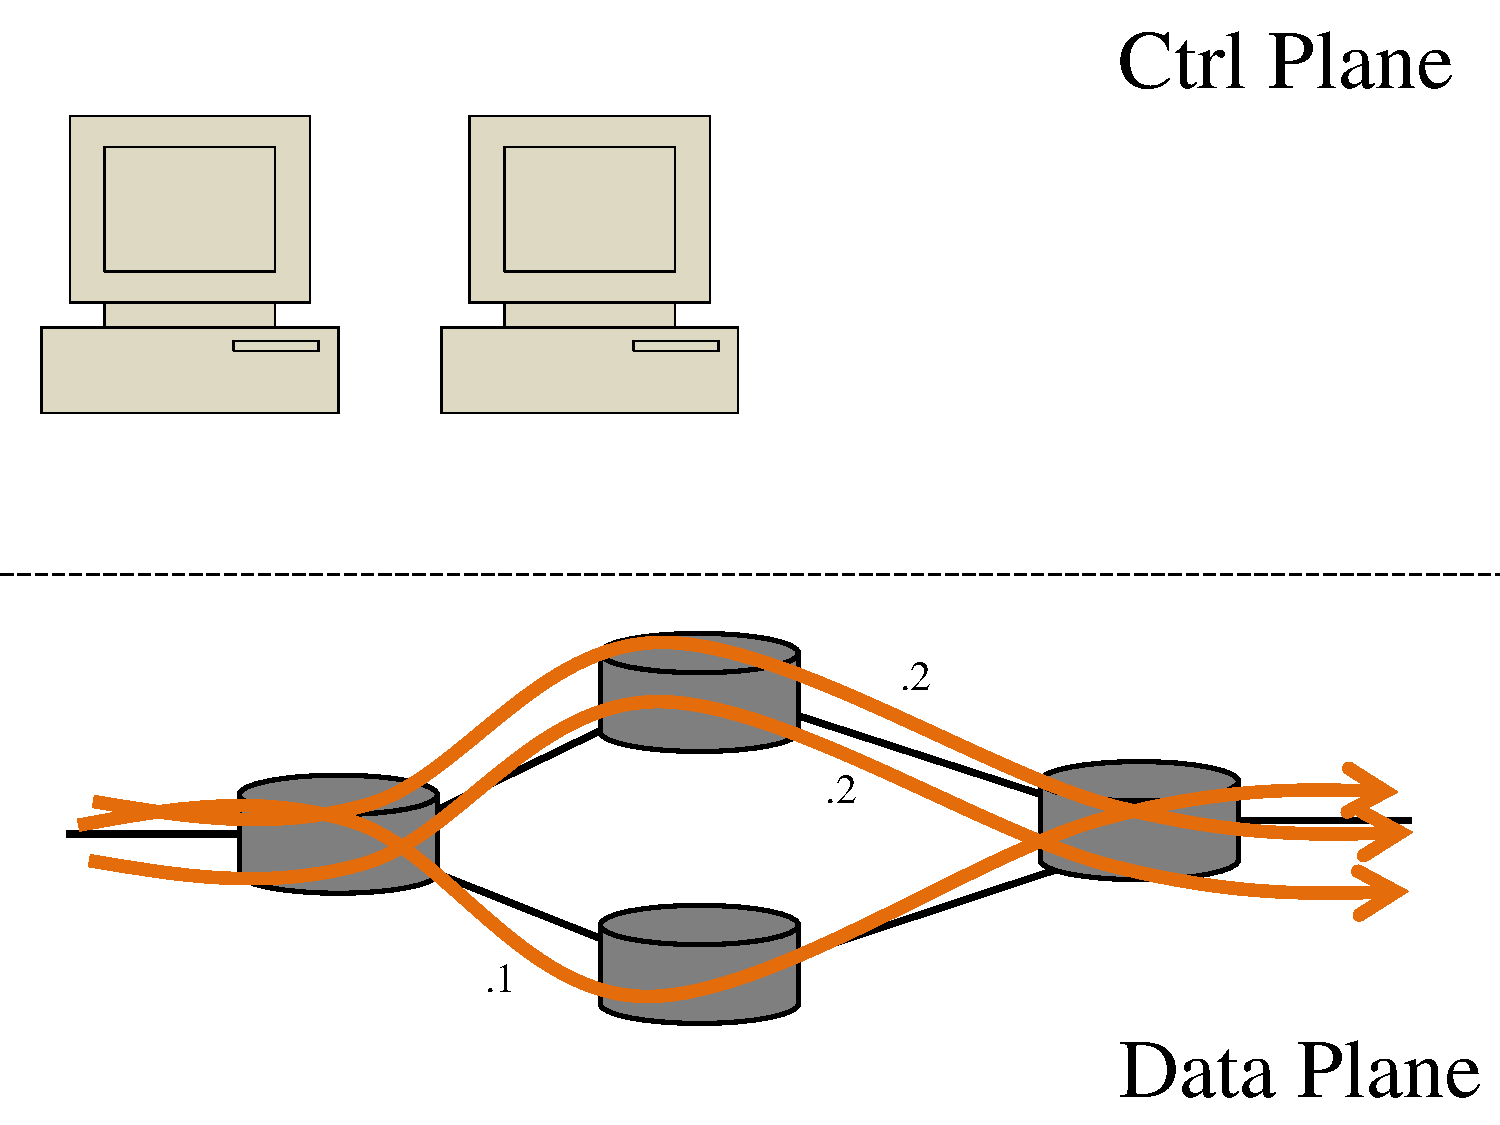
\includegraphics[width=0.35\columnwidth]{loadbal-before.pdf}~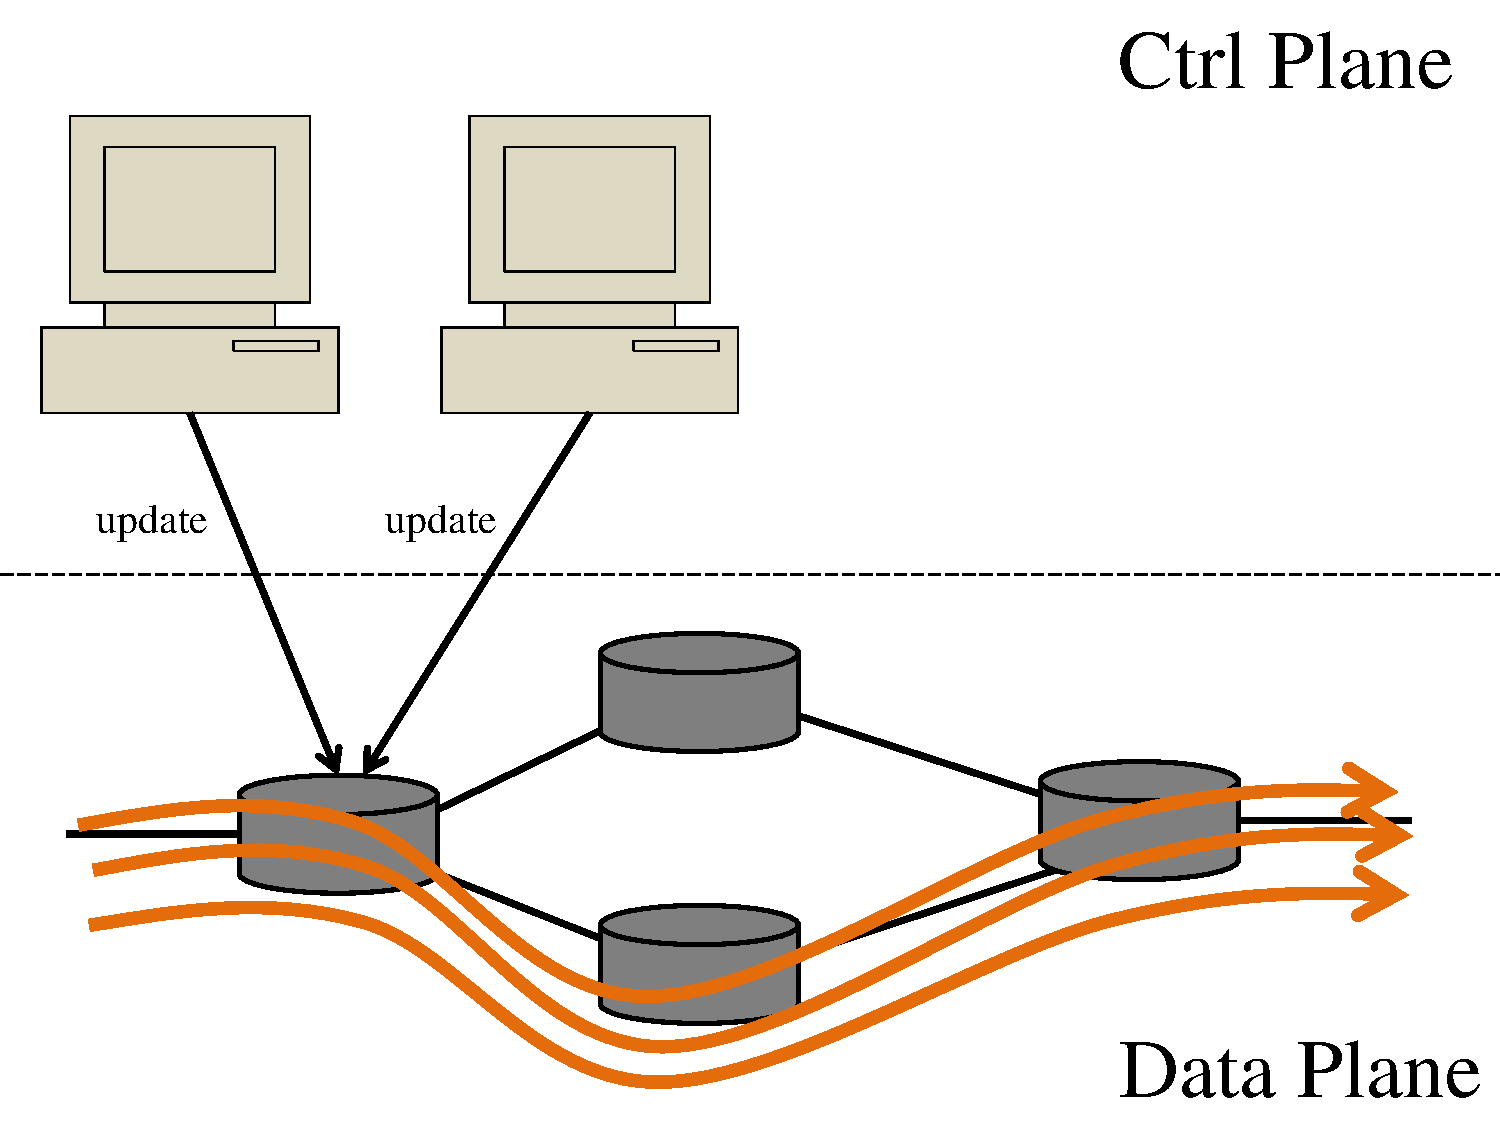
\includegraphics[width=0.35\columnwidth]{loadbal.pdf}~~
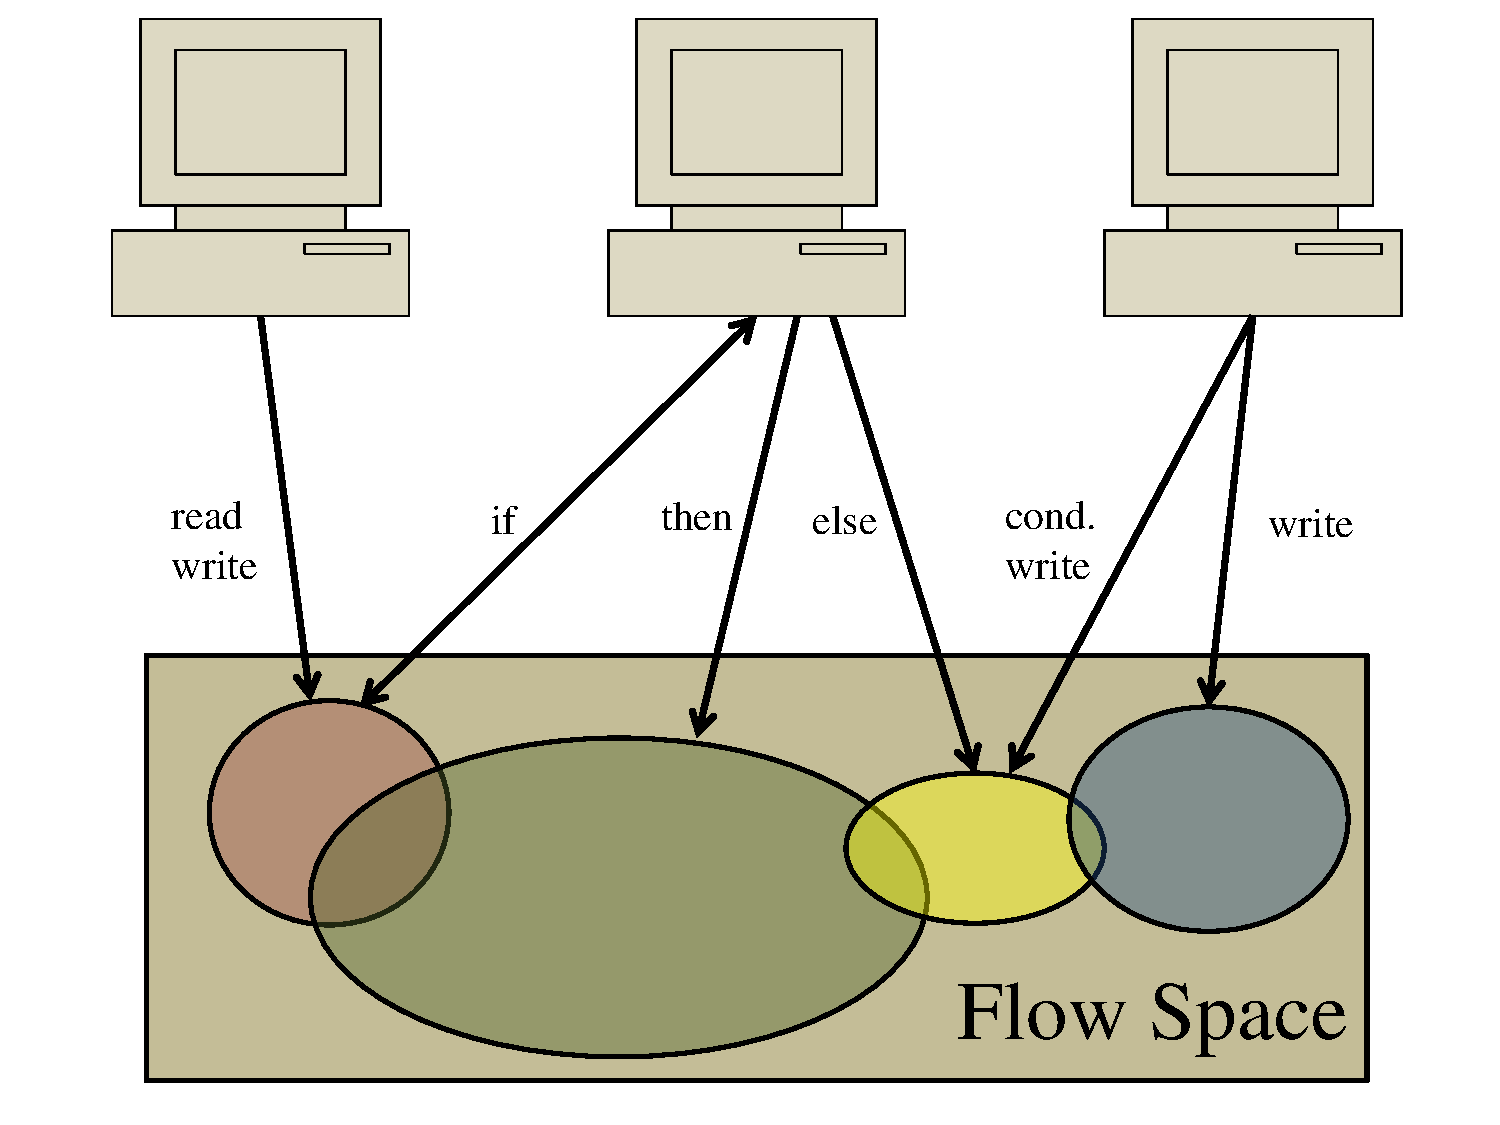
\includegraphics[width=0.8\columnwidth]{pic.pdf}\\
\caption{\emph{Left:} Load-balancing gone wrong. \emph{Right:} Illustration of transactional abstraction which  allows
controllers to modify switch configurations in complex ways,
and
depending on other flow spaces. Colors indicate different actions. \stefan{lets make two real transactions: one bundle and one 2 or 5 interactions?}}\label{fig:illu}
\end{figure*}

Finally, we remark that our solution is only based on flow tables
and does not make use
of group tables. 
Moreover, we do not make use of cookies: rules
are always identified by exact matches.

\section{Limitations and Motivation}\label{sec:motivation}

\stefan{liron, maybe we can discuss this section together: we need some more ideas}

Before presenting our transactional interface and implementation,
let us first discuss the limitations of the Openflow features discussed above.
At first sight, the bundle feature seems to provide everything
we need: it defines a sequence of read and write operations
 on the switch state which are executed atomically.
 However, such bundle transactions come with several
 limitations, as discussed in the following. Moreover,
 as we will see, our mechanism also does not \emph{need}
 the bundle feature. 

A bundle does not allow
 to change the switch state in any non-trivial way,
 as the read and write actions in the bundle do
 not support any conditional modifications or computations which
 depend on the read results. By leveraging
 the check overlap feature, it is at least possible
 to abort transactions depending on certain conditions
 in the overlapping
 flow spaces. However, in many cases, for example
 a load-balancing application,
 it can be interesting to define more general
 dependencies, which depend on, from a logical perspective,
 seemingly
 completely independent flow spaces,
 which however share the underlying physical network.
In other words, the bundle feature only allows us to
define ``one-shot transactions'',
transactions which do not support any further controller interactions.
Given
the limited computational options the Openflow interface of a switch offers,
it is difficult to implement more complex behavior.

\textbf{Example 1.} To give an example, let us consider a controller application in charge
of \emph{load-balancing}. The objective of the load-balancer
is to distribute flows equally across links or servers.
If multiple controllers concurrently and independently
update forwarding rules, they may unvoluntarily
unbalance the flow allocation. Note that this
is true independently of whether the flow spaces
affected by the respective controllers overlap or not.
More concretely, assume that two controllers concurrently
decide to forward traffic $1*$ and $0*$ to the same server.
Flow space overlap checks cannot be used to detect
such conflicts.
FIXME: make this example better


\begin{figure}[ht]
\centering
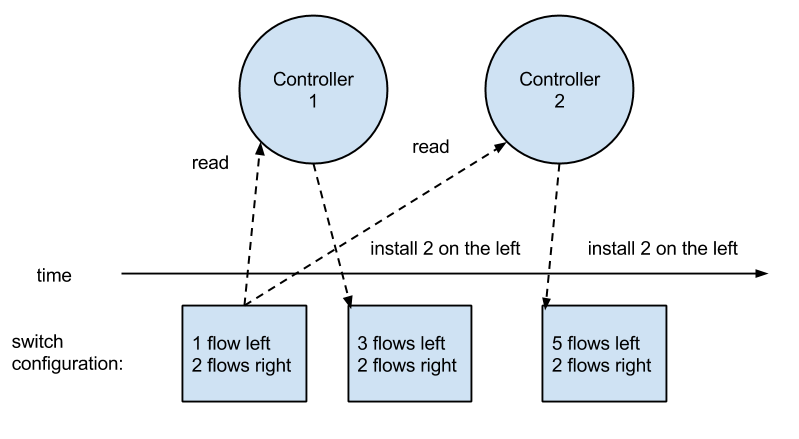
\includegraphics[width=1\columnwidth]{no-sync.png}\\
\caption{}\label{fig:no-sync}
\end{figure}

\begin{figure}[ht]
\centering
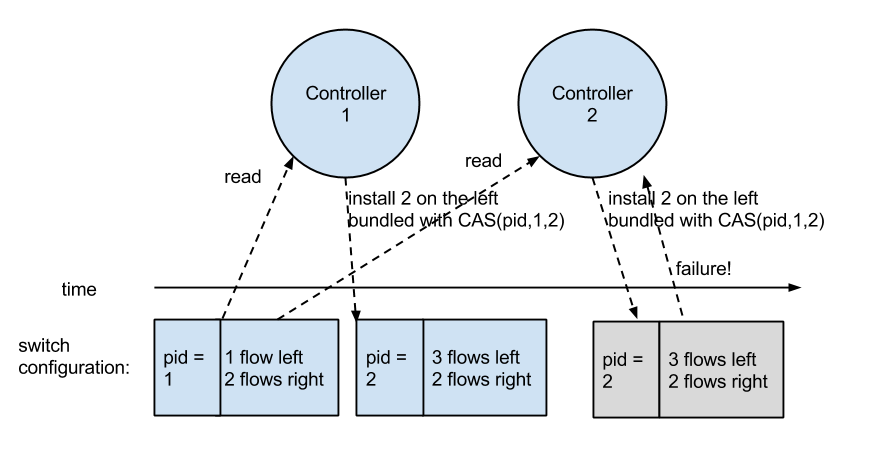
\includegraphics[width=1\columnwidth]{sync-with-cas.png}\\
\caption{}\label{fig:cas-sync}
\end{figure}

\textbf{Example 2.} To give another example,
consider the problem of modifying previously
installed forwarding policies.
While a bundle allows to conditionally add new rules or remove
old rules (and, using the flow space overlap
check, to abort the transaction if potentially conflicting
rules were already there), it cannot be used
to modify rules in non-trivial ways.
In other words, the bundle and overlap check only helps
for the conditional creation of rules, not their modification.

\stefan{It would be cool if we could make these examples more concrete,
at least one, and get back to it later again!}

%\section{The Container Object}\label{sec:vision}
\section{Transactional Synchronization}\label{sec:main}

This section describes how to introduce more powerful transactions.
Our implementation is based on two new synchronization objects,
allowing to coordinate controllers using identifiers.
At a high level, we export a
transactional interface which allows each controller $i\in[N]$ ($N\geq
2$) to perform multiple
operations on the configuration of an OpenFlow switch as an atomic
\emph{transaction}, inspired by the transactional-memory paradigm~\cite{stm-st95,tm-book}. A transaction may \emph{commit}, in
which case it appears as executed sequentially, or \emph{abort}, in
which none of its operations takes effect.

\subsection{Synchronization Objects}\label{sec:t-if}

We implement transactional access to  two kinds of objects: a read-write \emph{memory} abstraction
object, which we later use for storing the current used policy identifier, and a
\emph{resource-claimer} object, provides claiming a resource id (e.g. policy \emph{identifier}) in a
given (bounded or unbounded) set.
In theory one can use the memory abstraction to implement the resource claimer, 
however we found it far more simple and efficient to consider the resource claimer as base object.
%


A memory can be accessed with the following sequential
semantics:

\begin{itemize}
\item By performing $\textit{Write}(addr,k)$,
  $addr,k\in\Nat$, the value at memory offset $addr$ is set to $k$. For
  example, the offset $addr$ identifies the policy (identifier), 
  but our approach is more general.

\item $\textit{\compare}(addr,k)$, $addr,k\in\Nat$,
aborts current transaction if the value at memory offset $addr$ is not equal to $k$.
%returns $\textit{true}$ if and
%  only if $k$ is not currently claimed by any controller; if
%  $\textit{false}$ is returned, we say that the check operation
%  \emph{fails} (which causes an abort of the transaction invoking it).

\end{itemize}

Note that reading the memory can be done by just reading the switch configuration however such action doesn't affect the execution of the transaction (as $\textit{\compare}$ does).
As we will see, this abstraction can be implemented
without using the notion of bundles.

An immediate consequence of this memory interface is 
that we can implement a \emph{compare-and-set} (CAS) operation that takes two integer parameters
$\textit{old}$ and $\textit{new}$, reads the register and, if the
value of it is $\textit{old}$, replaces it with $\textit{new}$ and
returns $\textit{true}$; otherwise, $\textit{false}$ is returned and
we say that the CAS operation \emph{fails} (which causes an abort if
the transaction invoking it).


A resource-claimer object implements a weak type of locking, exports operations \emph{claim},
\emph{unclaim} and \emph{\claimcheck} with the following sequential
semantics:
%The container synchronization object introduced in this paper
%is essentially a transactional memory abstraction which can be implemented
%in standard Openflow switches.
%Before presenting the technical details in the next section,%
%we give a brief overview.

%The postulated container object can store an arbitrary number of \emph{items}.
%As we will see, these items correspond to flow entries on the Openflow switch.
%The same item may even exist multiple times in the container (i.e., the container
%is a multi-set).
%The container
%provides two main functions:
\begin{itemize}
\item by performing $\textit{claim}(k)$, $i\in[N]$,
  $k\in\Nat$, controller $i$ \emph{claims}
  identifier $k$;


\item by performing $\textit{unclaim}(k)$, $i\in[N]$, $k\in\Nat$, controller $i$
  \emph{unclaim} identifier $k$;

\item $\textit{\claimcheck}(k)$, $k\in\Nat$,
abort current transaction if $k$ is currently claimed by any controller.
%returns $\textit{true}$ if and
%  only if $k$ is not currently claimed by any controller; if
%  $\textit{false}$ is returned, we say that the check operation
%  \emph{fails} (which causes an abort of the transaction invoking it).

\end{itemize}

Again, none of these individual operations 
requires bundles.

\begin{comment}
\subsection{Interface}\label{sec:t-if}

\liron{this subsection doesn't flow well for me}

We assume that transactions may comprise operations on the flow table
of an SDN switch. Our transactional abstraction exports the
$\textbf{bundle}\{\;\ldots\;\}$ construct
containing a sequence of transactional
operations and may \emph{commit} and return responses to all its operations
or \emph{abort} (so that none of its operation takes effect).
We guarantee that in every execution, all committed
transactions constitute a \emph{legal} sequential
order~\cite{Pap79-serial}, i.e., every transaction appears as executed
sequentially. On the progress side, we ensure that a
transaction $T$ is only allowed to abort if either another
transaction updated a flow table entry read by $T$
or if one of $T$'s operations (\textit{check} or CAS) fails.
We employ the \emph{deferred-update} semantics:
no transaction can affect other transactions before it commits.
In particular, if a controller crashes before committing its
transactions, no future transaction can be affected.
%Note that
%, assuming such a transactional memory,
%a $\emph{contains}(x)$ operation can be implemented as a transaction
%composed of $\textit{cond-add}(x)$ followed by $\textit{cond-delete}(x)$.
%A \emph{set} abstraction is a special instance of a multi-set that is
%only modified with \textit{cond-add} and \textit{cond-delete}
%operations (this way the set only contains at most one copy of a given
%item).

\end{comment}


\subsection{Implementation}\label{sec:t-impl}

We now describe how to implement our transactional
abstractions using standard OpenFlow features.


\subsubsection{A resource claimer}
%features , including
%\emph{bundling}, \emph{conditional application}, and \emph{groups}.
%[[PK let us leave for the moment
%We will describe later how to implement some of these features
%in older Openflow versions where they are not
%supported. \textbf{TODO}
%]]
Algorithms~\ref{alg:claim}-\ref{alg:cas} describe implementations of
transactional operations  $\textit{claim}(x)$, $\textit{\claimcheck}(x)$, $\textit{unclaim}(x)$, $\textit{write}(x)$,  $\textit{\compare}(x)$
and $\textit{\cas}(x)$, respectively.
Algorithm~\ref{alg:commit} describes the procedure executed by
a transaction at \emph{commit time}.

We describe each operation as a message factory that returns OpenFlow commands that should be sent to the switch as part of the same transaction.
We assume that every transaction has a unique identifier  used to start a \emph{bundle}.
All messages generated during a transaction invocation, are wrapped by bundle messages carrying the bundle's id and followed by bundle commit message.
Messages with same bundle id are considered to belong to same bundle and are performed atomically.

%The OpenFlow messages that we use (besides )


Our implementation is based on OpenFlow flow entries modification command, the FlowMod message that we explain in Section \ref{sec:background}. We use the CHECK\_OVERLAP optional flag to make the transaction execution dependent on switch state.

We consider the match part of an entry to be a ternary string of bounded length (represented by binary value and mask) which can be applied to any set of supported packet header fields. In our implementation the $64$bit metedata field alone is suffice. Moreover we consider the action part of an entry to be an integer, which in practice can be implemented by a Set-Metadata instruction where the written value is that integer.

 As can be seen in Algorithms \ref{alg:claim}-\ref{alg:unclaim}, for the resource-claimer,
  the match part of the added flow entry represents the claimed id (id concatenated twice).
   In addition the mask part of the match (controller id concatenated with all-ones) varies from one controller to another in order to allow multiple controllers to claim the same number without overriding the same flow entry.
    We can see that for any two resource ids $x_1$ and $x_2$ and controller ids $c_1\neq c_2$ the match patterns $m_1=(x_1\concat x_1, c_1\concat all-1)$ and $ m_2=(x_2\concat x_2, c_2\concat all-1)$ are not equal even if $x_1=x_2$ therefore they can both be used to claim and unclaim without affecting each other.

In order to check if a number is claimed we try to create the corresponding entry while setting the
flag \textsf{CHECK\_OVERLAP} and using different action ($2$ instead of $1$), thereby inflicting a failure in case an entry with overlapping match value exists. If the check succeeds we delete the entry. Considering $m_1$ and $m_2$ defined above and their respective actions $a_1=x_1\concat c1$ and $a_2=x_2\concat c2$,  they overlap with different actions iff $x_1=x_2$. Therefore if one is used in \claimcheck after the other used in claim, a conflict is detected iff $x_1=x_2$, as expected.

Note that for switch space reasons, checking for claims contains also a deletion of the added tester flow entry but it has no affect on claims and checks of other controllers and therefore the deletion command doesn't have to be sent as part of a bundle. This makes the \textsf{\claimcheck} operation atomic by nature, similar to the \textsf{claim} and \textsf{unclaim}, as being implemented by essentially one command.



%A container contains items: they represent the flow table entries (i.e., a match-action rules, plus e.g., counters belonging to the rule).
%Items can be added and removed atomically and in bundles (e.g., to update the switch with
%a new policy). Recall that we want to add items only if they do not exist
%yet; otherwise the transaction should abort without taking effect.
%And similarly for removes: transactions should not take effect if the corresponding
%update contains rules which currently do not exist at the switch.

\begin{algorithm}[H]
    \caption{$\textit{claim}(x)$}
    \label{alg:claim}
    \begin{algorithmic}[1]
    \Require \emph{self} as the calling controller id.
%    \Ensure
    		\State $value \gets x\concat x$
    		\State $mask \gets self\concat all-1$
	    	\State $match \gets (value,mask)$
    		%\State $cookie \gets x\concat self$
    		\State $action \gets 1$
    		\State $flag \gets 0$
    		\State $cmd\gets \textsc{FlowMod}(match, op = ADD, flag, action) $
			\Return $cmd$
    \end{algorithmic}
\end{algorithm}

\begin{algorithm}[H]
    \caption{$\textit{\claimcheck}(x)$}
    \label{alg:check}
    \begin{algorithmic}[1]
    \Require \emph{self} as the calling controller id.
%    \Ensure
    		\State $value \gets x\concat x$
    		\State $mask \gets self\concat all-1$
    		\State $match \gets (value,mask)$
    		%\State $cookie \gets x\concat self$
    		\State $action \gets 2$
    		\State $flag \gets \textsf{OFPFF\_CHECK\_OVERLAP}$
    		\State $cmd1\gets \textsc{FlowMod}(match, op = ADD, flag, action) $
    		\State $cmd2\gets \textsc{FlowMod}(match, op = DELETE) $
			\Return $cmd1$,$cmd2$
    \end{algorithmic}
\end{algorithm}

\begin{algorithm}[H]
    \caption{$\textit{unclaim}(x)$}
    \label{alg:unclaim}
    \begin{algorithmic}[1]
    \Require \emph{self} as the calling controller id.
%    \Ensure
    		\State $value \gets x\concat x$
    		\State $mask \gets self\concat all-1$
    		%\State $cookie \gets x\concat self$
    		\State $match \gets (value,mask)$
    		\State $cmd\gets \textsc{FlowMod}(match, op=DELETE) $
    	
			
			\Return $cmd$
    \end{algorithmic}
\end{algorithm}

\subsubsection{A memory abstraction}


We use similar techniques for implementing memory \memwrite and \compare
 operations.
 As can be seen in Algorithms \ref{alg:write}-\ref{alg:compare},
  the match part of the added flow entry is used as the memory address and the action as the written value. Values written to the same address will replace one another, following the command definition to replace old flow entry with a new one in case they share the same match parts (as described in Section \ref{sec:background}).

In order to check if a value is written in a given address, we try to add it the same way as in the \memwrite operation  but we also set the \textsf{CHECK\_OVERLAP} flag. If the value is not there, our action differ from the action of the existing entry thereby inflicting a failure.
In case the value is there, our flow entry replaces the existing flow entry with identical one.
In addition we present in Algorithm \ref{alg:cas} a simple implementation of Compare and set (CAS) using the two last operations.

\begin{algorithm}[h]
    \caption{$\textit{write}(addr,k)$}
    \label{alg:write}
    \begin{algorithmic}[1]
    %\Require  id $i$.
%    \Ensure
    		\State $value \gets addr$
    		\State $mask \gets  all-1$
    		\State $match \gets (value,mask)$
    		%\State $cookie \gets x\concat self$
    		\State $action \gets k$
    		\State $flag \gets 0$
    		\State $cmd\gets \textsc{FlowMod}(match, op = ADD, flag, action) $
			\Return $cmd$
    \end{algorithmic}
\end{algorithm}

\begin{algorithm}[h]
    \caption{$\textit{\compare}(addr,k)$}
    \label{alg:compare}
    \begin{algorithmic}[1]
    %\Require  id $i$.
%    \Ensure
    		\State $value \gets addr$
    		\State $mask \gets  all-1$
    		\State $match \gets (value,mask)$
    		%\State $cookie \gets x\concat self$
    		\State $action \gets k$
    		\State $flag \gets \textsf{OFPFF\_CHECK\_OVERLAP}$
    		\State $cmd\gets \textsc{FlowMod}(match, op = ADD, flag, action) $
			\Return $cmd$
    \end{algorithmic}
\end{algorithm}



\begin{algorithm}[h]
    \caption{$\textit{\cas}(addr, old,new)$}
    \label{alg:cas}
    \begin{algorithmic}[1]
    %\Require  id $i$.
%    \Ensure

    		\State $cmd1\gets \textsc{\compare}((addr, old) $
    		\State $cmd2\gets \textsc{\memwrite}((addr, new) $
			\Return $cmd1,cmd2$
    \end{algorithmic}
\end{algorithm}



\section{Discussion of Use-Cases}\label{sec:apps}

More powerful transactions can be useful in many scenarios.
Let us revisit our examples from earlier: with
transactions we can easily solve the load-balancing
and rule modification problem.
In the following we give two more examples of our approach.

\subsection{Policy Updates}

\stefan{liron: maybe we can make a more concrete example like we had it in medieval?}

Our first example (Algorithm~\ref{alg:simple-update}) is a simple policy composition protocol that
allows a set of  controllers to concurrently update switch  \emph{policies} , i.e., sets of
effective rules in its flow tables, under the
condition that these rules can be composed with the currently installed
policy (the composition predicate is encoded in a user-specific
$\textit{apply\_update}()$ function~\cite{cpc}.

Every policy is associated with a \emph{policy identifier}.
In the algorithm, the controller first reads the currently installed
policy, then choose a new unique policy, checks whether the new
policy and the current policy can be composed and, if so, replaces the
current policy with the composition. If, meanwhile, a new
policy (with a different identifier) has been installed, the update
fails and takes no effect.

Algorithm~\ref{alg:simple-update} use increasing numbers as policies
ids and use them in order to make sure that the new policy, with id
$x$, replaces the (what considered as) current policy, with id
$x-1$. Considering the policies ids, we send the policy installation
commands as part of a bundle that also tries to perform
$CAS(x-1,x)$, thereby insuring that the commands are
performed iff the current policy is still there and preventing other
controllers to replace the new policy with another without observing it.

For brevity, we omit explicitly putting the $\textbf{bundle}\{...\}$ construct
around each of the transactional operation used in the algorithm.
Indeed, since \textit{claim} and \textit{unclaim} operations cannot
cause the corresponding transaction, we can assume that all
``singleton'' (consisting of one operation only)  transactions
containing such operations always commit.

Algorithm~\ref{alg:simple-update} allows policy identifiers to grow
without bound. In fact, as was observed in~\cite{cpc}, the number of currently
used policies can be made proportional to the number of concurrent
controllers.


 It takes a set of rules $U$ (not yet a policy)and proceeds as follows: first, we seek to
 obtain a unique \emph{id}. FIXME: to be continued...
 \textbf{LS: I am not sure if I need to tell every step of the story or maybe it best to explain the main dif from the previous one similarly to what I just wrote next}.

Algorithm~\ref{alg:update} claims the current policy id in order to prevent someone of using it with different policy in the future (during the current update) and in the bundle used to update the policy it also checks that the new policy id that it about to use (chosen from a finite set of ids) wasn't claimed by someone else.

\hide{
We compute our new suggested policy by applying the update requests on top of current policy, supporting any kind of requests and policies. Then we make a transaction (using the bundle feature) to atomically check that our policy id is not blocked by anyone else, to change the current policy id to ours (an action that would fail if the current policy id is no longer what we are counting of) and to actually configure our new policy.

If one of the actions in the transaction fails we try again. There is no progress guaranty for each controller but there is one for the whole system - at least one of the controller will succeed in fulfilling its update requirements.
}



\textbf{TODO: fix the pseudocode, make the use of afdd/delete
  operations uniform, make all switch operations transactional}

\liron{for alg \ref{alg:simple-update} we should say that switch configuration = pid + policy}

\begin{algorithm}[t]
    \caption{Policy update with only CAS}
    \label{alg:simple-update}
    \begin{algorithmic}[1]
    \Require unsafe policy update function $U$, a predefined switch (memory) address for policy id: $pid\_addr$
    \Ensure installed policy is consistent with previous one
 		%\Do
 		\Repeat
 			\State $pid,policy\gets$ \textbf{read} switch configuration
 			\State $cmds\gets U(policy)$
 			\startTxn
	 			\State $CAS(pid\_addr,pid,pid+1)$
	 			\State \textbf{send} $cmds$ %conditioned on $metadata=my\_a$
	 			%\State update policy selector to $my\_a$
 			\endTxn
     		%\State $res \gets $ commit transaction
     	\Until{$res\neq\texttt{abort}$}
     	%\doWhile{$res=False$}
%   \vspace{3mm}
			\Return

    \end{algorithmic}
\end{algorithm}


\liron{for alg \ref{alg:update} we should say that switch configuration = pid + claims + policy}

\begin{algorithm}[t]
    \caption{Advanced policy update}
    \label{alg:update}
    \begin{algorithmic}[1]
        \Require unsafe policy update function $U$, a predefined switch (memory) address for policy id: $pid\_addr$, a predefined id space $C$.
    \Ensure installed policy is consistent with previous one
 		%\Do
 		\Repeat
		 	\State $pid,claims,policy\gets$ \textbf{read} switch configuration
 			\State $claim(pid)$
 			\State $pid2,claims,policy\gets$ \textbf{read} switch configuration
 			\If {$pid\neq pid2$}
	 			\State $unclaim(pid)$
 				\State {\bf continue} (\textbf{restart} loop)
 			\EndIf
 			\State $my\_id\gets$ choose a number from $C\setminus claims$
 			\State $cmds\gets U(policy)$
 			\startTxn
 				\State $\claimcheck(my\_id)$
	 			\State $CAS(pid\_addr, pid,my\_id)$
	 			\State \textbf{send} $cmds$ %conditioned on $metadata=my\_a$
	 			%\State update policy selector to $my\_a$
 			\endTxn
	 		\State $unclaim(pid)$
     		%\State $res \gets $ commit transaction
     	\Until{$res\neq\texttt{abort}$}
     	%\doWhile{$res=False$}
%   \vspace{3mm}
			\Return

    \end{algorithmic}
\end{algorithm}



\subsection{Consensus and Replicated State Machines}

It is straightforward to implement consensus among the controllers
using just a single register that can be accessed with an atomic CAS
operation~\cite{Her91}. In our transactional setting, the controllers
can use CAS to replace the default value of such a register
with their consensus input values (e.g., the identifiers of the
policies that should be applied first). If the corresponding
singleton transaction commits, the controller consideres itself
the \emph{winner} and decides on its input, if
it aborts (the controller fails in the CAS) it remains to read the register to get the input of the
winner to decide.

By using multiple CAS invocations, the controllers can implement any
generic replicated state machine~\cite{Her91,Lam98}, which will be instrumental in the
next section.

Given the CAS, we can also implement more complex operations,
for example the replicated state machine postulated in STN~\cite{stn}:
in order to choose tags in a consistent manner, CAS needs to be enhanced
with a notion of tags. 

%\paragraph{One-Shot Update} FIXME: desribe how to implement one-shot update
%
%\paragraph{STN}
%
%\textbf{TODO}
%

\begin{comment}
\section{In-Band Composition}\label{sec:compo}

We conclude our technical contribution by showing that sometimes,
powerful synchronization mechanisms can be implemented
in-band \emph{even without bundles}.
Concretely, we show that sometimes it is even possible
to automatically compose updates originating from different controllers,
in-band and just using Openflow.

To illustrate this point, we consider a simple example
with two controllers concurrently issuing updates to a single
given switch.

FIXME: Explain, maybe even with an example?

\begin{figure}[t]
\centering
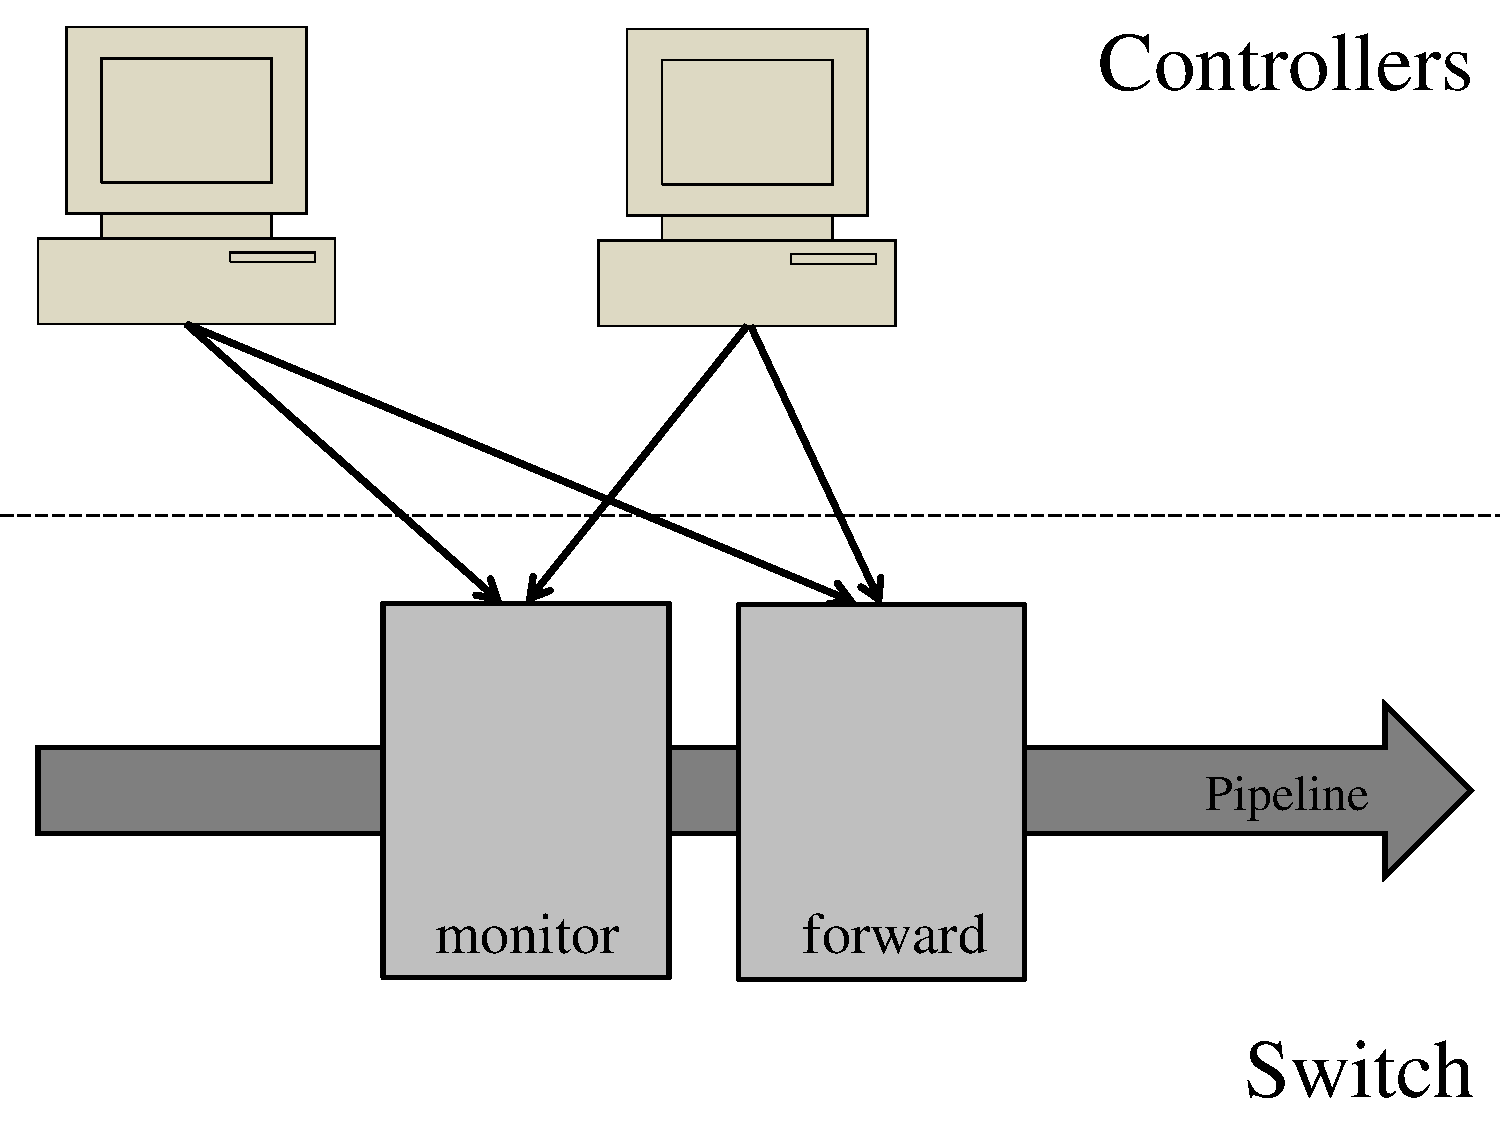
\includegraphics[width=0.8\columnwidth]{composition.pdf}\\
\caption{Composition.}\label{fig:illu}
\end{figure}

\end{comment}

\begin{comment}

\section{Transactions in Openflow}\label{sec:sync}

Multi-write and read-modify transactions.

\subsection{Dealing with multiple updates}

TBD - adding the notion of versions and cleanup/GC. probably no good way to solve infinite versions... maybe check literature on shared memory and multiple writes.


\subsection{Improving the scheme with check-overlap}\label{sec:todo}

Till now we considered a model that allows multiple updates to match-action entries. Here we extends the model with actions create-entry and delete-entry that may failed and abort the whole transaction depending on the existence on non-existence of specific entries prior to the action.
%TBD - much less resources. easily solving the infinite versions issue.

Next we show how such actions can be used to implement consensus with much less resources. We use entry id as a property used to reference specific entry.

\section{Applications and ramifications}\label{sec:application}



\section{The Underlying Theory}\label{sec:background}

idea: multi-write consensus, a not well-known result!

In order to solve consensus we suggest to use the atomic multiple entries update capability (which is discussed in Openflow standard). A shared memory system that supports atomic write to (enough) multiple locations is known to allow the implementation of consensus objects. For example consider the following implementation utilizing $n^2$ memory locations, $M_{i,j}$, where $i,j\in[n]$, and the suggested values $\{v_i\}_{i\in [n]}$. All locations are initialized to zero.

In order to participate, a server i, writes its suggested value $V_i$ and atomically rewrites row i ($M_{i,*}$) with value "1" and column i ($M_{*,i}$) with value "2". After the atomic write, a server $i$ first reads the diagonal ($M_{j,j}$ for $j\in [n]$), and consider all observed servers as candidate set S.  Then server i reads all candidates intersections (locations $M_{j,k}$ where $j,k\in S$. And computes the winner server id w that was overwritten by all other candidates, i.e. such that $M_{w,k}=2$ for all $k\in S {w}$. The consensus value is $v_w$.
Note that a snapshot could replace the two reading phases.



\section{Basic One-Touch Mechanism}\label{sec:realization}

We address the problem of committing consistent policies to SDN switch concurrently by multiple controllers.
We show that assuming minimalistic control protocol, SDN switch configuration space can be used to implement a consensus object thereby allowing controllers to agree on each next policy update.

\subsection{SDN switch configuration space as shared memory}





Our first observation is that a match-action configuration which is accessed by multiple controllers can be considered as shared memory. Note however that standard memory map and index/offset to a word, while Flow Table entries are not necessarily indexed. However, we assume that each flow entry has some property that allows the operator to specifically reference and update it, for example Openflow entry's cookie. In cases where this property value can't be determined by the operator, we can use other variable entry properties to store the index, for example we can represent memory value $v$ in offset $i$ by an match-action entry whose match is $in\_port = i$ and action is "forward port $x$".
%To overcome this we can use the match part of an entry as the index and the action part as the word value.


Going back to the policy update problem, the consensus scheme allow all servers to decide on next policy by using consensus value as policy identifier, and writing the policy in advance. However this scheme doesn't actually apply the policy on incoming packets and it remains to configure the switch according to the next policy once it is decided. Making this scheme fail safe (handling failure of winning server) can be ensured by allowing any server to reconfigure the switch.

\subsection{ One-Touch}

In some scenarios it may be desirable to shorten the policy update time by avoiding the consensus reading and policy configuration step. We define this as the one touch policy update, namely we require each server to contact the switch only once in order to (try and) update the policy, in other words participating in reaching consensus and applying it with one atomic write. Solving this problem also has significance in understanding the strength of the SDN switch computation model.

The main idea of our solution is to adjust the previous policy update scheme in a way that performs consensus validation phase during every packet processing thereby requiring the servers only to make the first phase of the consensus - atomically writing the matrix.
In order to allow the packets to validate the consensus we make the following observation: while servers can be abstracted as memory writers, the packets processed by the switch are the readers. Openflow standard define an atomic write transaction as being atomic in relation to the processed packets thereby making packet processing a multiple read transaction but one read location per table is allowed. This means that if each memory location used in the consensus scheme will be stored in different table then each packet will be able to read all of them.

However, reading each memory location is not enough, as the scheme requires to make a validation that involves multiple values. We utilize the metadata field in order to store all read values, in more details, each memory value $M_{i,j}$ is stored in offset i+j*n in the metadata field. Once all values are in the metadata field, we can detect the consensus winner by trying different matches on the metadata. Although we can have one match entry per possible matrix state, this solution requires exponential number of entries. A better way which we describe next requires only $O(n^2)$ entries utilizing n tables.

Our compact validation use additional temp variable, $temp_winner$, to hold the current best consensus candidate. Each of the n validating tables checks different "column" in the matrix and update $temp_winner$ to keep track of the winner so far (after examining a prefix sub set of the columns). The entry t in table k $(0<=k<n)$  matches the case where current winner=t and location $(t,k)$ in the matrix (packet header) equals 1 and location (k,k) is non-zero. After all validating tables are processed, $temp_winner$ stores the id of the winning server which can be used to match on its policy rules (filtering out other policies) or to use the goto table command to jump to a designated policy table of the server.


\section{The Practical Implementation}\label{sec:extension}

\end{comment}

\section{Related Work}\label{sec:relwork}

There exists a wide consensus that SDN control planes need to be distributed.~\cite{onos,onix,elasticon}
Onix~\cite{onix} is one of the earliest proposals, and introduced the
the notion of Network Information Base (NIB), abstracting network state
distribution from control logic, but
requiring mechanisms for the detection and resolution of conflicts.
Also spatially distributed control planes to improve scalability and
latency have been studied intensively
in the literature~\cite{kandoo,ctrl-place,hotsdn13loc}
proposes an elastic distributed controller architecture.

Operating and updating SDNs consistently is already non-trivial
from the perspective of a single controller. Reitblatt et al.~\cite{network-update}
introduced the notion of
per-packet consistency and proposed a 2-phase update protocol based on tagging.
%, and described the \emph{two-phase update} technique, also used in our algorithms.
Mahajan and Wattenhofer~\cite{roger-hotnets} considered weaker transient
consistency guarantees, and proposed more efficient network update algorithms
accordingly. Ludwig et al.~~\cite{hotnets14update} studied algorithms for secure
network updates where packets are forced to traverse certain waypoints or
middleboxes. Ghorbani et al.~~\cite{correct-virt} recently argued for the design
of network update algorithms that provide even stronger consistency guarantees.

To the best of our knowledge, the only paper explicitly addressing the consistent
network update problem from a distributed-controllers perspective is STN~\cite{stn}:
STN provides a transactional interface offering all-or-nothing semantics and serializability
(the ``holy grail'' of safety properties), allowing
controllers to install policies in a conflict-free manner; if some controllers fail,
other controllers can take over. STN~\cite{stn} is based on
atomic read-modify-write primitives provided by the switches, but
while the availability of such primitives is postulated, no implementation is
described. In this paper, we provide this missing link, and also show that other useful and
more powerful synchronization primitives can be implemented.
Also, some STN implementations in~\cite{stn} assume that the control
plane maintains a certain amount of synchrony that allows controllers
to solve consensus or implement a replicated state machine.
In this paper, we describe an OpenFlow-based consensus protocol that
can be used for this purpose.

Our work is also closely related to the recent work on providing more high-level
abstractions and programming languages for SDNs, such as Frenetic~\cite{frenetic},
also enabling policy composition~\cite{pyretic}. Our work complements these works
on programming abstractions
by initiating the discussion of concurrency objects and abstractions.

The transactional interface we describe in this paper is inspired by the
work on speculative concurrency control using software transactional memory
(STM)~\cite{stm-st95,tm-book}.
%[[PK I think this is enough]]

Our work also contributes to the ongoing discussion of what can be implemented
in-band in Openflow~\cite{compute,reclaim}, by assuming the relevant perspective of distributed
synchronization.

\hide{
In terms of distributed computing: TODO PETR: maybe modify a bit the text below
and also write more about multi-writer consensus etc.?

\noindent\textbf{Distributed Computing.}
There is a long tradition of defining correctness of a concurrent system via
an equivalence to a sequential one~\cite{Pap79-serial,Lam79,HW90}.  The notion
of sequentially composable histories is reminiscent of
linearizability~\cite{HW90}, where a history of operations concurrently
applied by a collection of processes is equivalent to a history in which the
operations are in a sequential order, respecting their real-time precedence.
In contrast, our sequentially composable histories impose requirements not
only on high-level invocations and responses, but also on the way the traffic
is processed. We require that the committed policies constitute a
conflict-free sequential history, but, additionally,  we expect that each
\emph{path} witnesses only a prefix of this history, consisting of all
requests that were committed before the path was initiated.
%
The transactional interface exported by the CPC abstraction is inspired by the
work on speculative concurrency control using software transactional memory
(STM)~\cite{stm-st95}.
%, thus the  term \emph{software transactional networking}.
Our interface is however intended to model realistic network
management operations, which makes it simpler than recent
dynamic STM models~\cite{dstm}.
%In particular, the sets of rules to be installed by a policy update do not depend on the state of the
%network.

Extending the interface to dynamic policies that adapt their behavior based on
the current network state sounds like a promising research direction.  On the
other hand, our criterion of sequential composability is more complex than
traditional STM correctness properties in that it imposes restrictions not only
on the high-level interface exported to the control plane, but also on the
paths taken by the data-plane packets.
Also, we assumed that controllers are subject to failures, which is usually not
assumed by STM implementations.
}

\section{Conclusion}\label{sec:conclusion}

While much progress has been made over the
last years in the development of more intuitive programming
languages for SDNs (e.g., Frenetic, Pyretic, Merlin), the
question of which synchronization abstractions to provide
has received much less attention.
%
In this paper, we describe transactional abstractions that
can be implemented using standard Openflow features.
%
Our work complements existing research on the design of
distributed control planes, and also provides some missing links,
e.g., for the transactional approach taken by STN~\cite{stn}.
We also hope that our work can nourish the discussion of
which synchronization objects we can and want to implement
in an SDN.


{
\bibliographystyle{abbrv}
\bibliography{references}  % main.bib is the name of the Bibliography in this case
}

\cleardoublepage

\onecolumn

\begin{appendix}

\section{The FlowMod Command}

\lstset{% general command to set parameter(s)
	basicstyle=\small, % print whole listing small
	keywordstyle=\color{black}\bfseries, % underlined bold black keywords
	identifierstyle=, % nothing happens
	commentstyle=\color{mygrey}, % white comments
	stringstyle=\ttfamily, % typewriter type for strings
	showstringspaces=false, % no special string spaces
	language=C}
\begin{lstlisting}
struct ofp_flow_mod {
	struct ofp_header header;
	uint64_t cookie; /* Opaque controller-issued identifier. */
	uint64_t cookie_mask; /* Mask used to restrict the cookie bits
		that must match when the command is
		OFPFC_MODIFY* or OFPFC_DELETE*. A value
		of 0 indicates no restriction. */
	/* Flow actions. */
	uint8_t table_id; /* ID of the table to put the flow in.
		For OFPFC_DELETE_* commands, OFPTT_ALL
		can also be used to delete matching
		flows from all tables. */
	uint8_t command; /* One of OFPFC_*. */
	uint16_t idle_timeout; /* Idle time before discarding (seconds). */
	uint16_t hard_timeout; /* Max time before discarding (seconds). */
	uint16_t priority; /* Priority level of flow entry. */
	uint32_t buffer_id; /* Buffered packet to apply to, or
		OFP_NO_BUFFER.
		Not meaningful for OFPFC_DELETE*. */
	uint32_t out_port; /* For OFPFC_DELETE* commands, require
		matching entries to include this as an
		output port. A value of OFPP_ANY
		indicates no restriction. */
	uint32_t out_group; /* For OFPFC_DELETE* commands, require
		matching entries to include this as an
		output group. A value of OFPG_ANY
		indicates no restriction. */
	uint16_t flags; /* Bitmap of OFPFF_* flags. */
	uint16_t importance; /* Eviction precedence (optional). */
	struct ofp_match match; /* Fields to match. Variable size. */
	/* The variable size and padded match is always followed by instructions. */
	//struct ofp_instruction_header instructions[0];
		/* Instruction set - 0 or more. The length
		of the instruction set is inferred from
		the length field in the header. */
};
\end{lstlisting}


- Creating an entry with the same match part replaces the existing one.

\section{Bundle Control Message}

%/* Message structure for OFPT_BUNDLE_CONTROL. */
\begin{lstlisting}
struct ofp_bundle_ctrl_msg {
	struct ofp_header header;
	uint32_t bundle_id; /* Identify the bundle. */
	uint16_t type; /* OFPBCT_*. */
	uint16_t flags; /* Bitmap of OFPBF_* flags. */
	/* Bundle Property list. */
	struct ofp_bundle_prop_header properties[0]; /* Zero or more properties. */
};
\end{lstlisting}

\begin{lstlisting}
* Adding a message in a bundle is done with. */
struct ofp_bundle_add_msg {
	struct ofp_header header;
	uint32_t bundle_id; /* Identify the bundle. */
	uint16_t pad; /* Align to 64 bits. */
	uint16_t flags; /* Bitmap of OFPBF_* flags. */
	struct ofp_header message; /* Message added to the bundle. */
	/* If there is one property or more, 'message' is followed by:
	* - Exactly (message.length + 7)/8*8 - (message.length) (between 0 and 7)
	* bytes of all-zero bytes */
	/* Bundle Property list. */
	//struct ofp_bundle_prop_header properties[0]; /* Zero or more properties. */
};
\end{lstlisting}

\section{To Be Deleted...}

\begin{algorithm}[h]
    \caption{Policy composition without bundle}
    \label{alg:wobundle}
    \begin{algorithmic}[1]
    \Require policy $P$ (a set of FlowMod entry creation commands), three consecutive flow tables ids (per controller) $T_s,T_0,T_1$, active table index $active\in\{0,1\}$.
    %\Ensure installed policy is consistent with previous one
    \State $unactive \gets active + 1 \mod{2}$
    \For {$cmd \in P$}
	    \State $cmd.action\gets Reencode(cmd.action)$
	    \State $cmd.table\_id\gets T_{unactive}$
	    \State send $cmd$
    \EndFor
    \State modify the action of $T_s$ entry to goto $T_{unactive}$
    \State clear table $T_{active}$
    \State $active \gets unactive$
	\Return

    \end{algorithmic}
\end{algorithm}

\begin{algorithm}[h]
    \caption{Update with pipeline}
    \label{alg:pipeline}
    \begin{algorithmic}[1]
    \Require update requirements $U$, array $ARR$.
    \Ensure installed policy is consistent with previous one
			\Return

    \end{algorithmic}
\end{algorithm}


\begin{comment}
\section{Implementing CAS with FlowMod commands}\label{sec:without-groups}
This section describes an implementation without group tables.

Here we describe a second implementation of the Compare\&Set abstraction that is based on entirely on flow entry creations and deletions (FlowMod commands).

The CHECK\_OVERLAP flag enables us to add an entry if no contradicting entry exists and to fail if such do exists. However, the compare stage of \cas requires us to fail if a certain value doesn't exists, i.e. $\cas(x,y)$ failes iff $x \notin T$, where $T$ is the set of match entries defined in a dedicated flow table.
...
...


\begin{algorithm}[H]
    \caption{$\textit{CAS}(old,new)$}
    \label{alg:cas2}
    \begin{algorithmic}[1]
    %\Require  id $i$.
%    \Ensure
			\State $cmds \gets new\ list()$
    		\State $value \gets  old$
    		\State $mask \gets  all-1$
    		\State $match \gets (value,mask)$
    		%\State $cookie \gets x\concat self$
    		\State $action \gets 2$
    		\State $flag \gets OFPFF\_CHECK\_OVERLAP$
    		\State $cmd1\gets \textsc{FlowMod}(match, op = ADD, flag, action) $
    		\State $cmd2\gets \textsc{FlowMod}(match, op = DELETE) $
    		\State $cmd3\gets \textsc{FlowMod}(cookie = old, op = DELETE) $
    		\State $cmds.append(cmd1)$
    		\State $cmds.append(cmd2)$
    		\State $cmds.append(cmd3)$
    		\State $range\_matches \gets EncodeRange([0,new-1])\cup EncodeRange([new+1,MAX\_ID])$
    		\For {$r\_match \in range\_matches $}
    		    		\State $cookie \gets new$
    		    		\State $action \gets 1$
    		    		\State $flag \gets 0$
    		    		\State $cmd\gets \textsc{FlowMod}(r\_match, ADD, flag, cookie, action) $
    		    		\State $cmds.append(cmd)$
    		\EndFor
			\Return $cmds$
    \end{algorithmic}
\end{algorithm}



\section{Implementing CAS with GroupMod commands}\label{sec:with-groups}
Similarly, we use a deletion of group $x$ and a creation of group $y$ (with GroupMod commands) as an
abstraction to performing a $CAS(x,y)$ operation to a special $16$bit register (we abstract only one register). The $16$ bit limit is resulted by th $16$bit group id size.
%The group id of the added group represents the added number.
Note that trying to delete a group that doesn't exist (or trying to create a group with id that already exists) fails, thereby preventing adding the new value $y$ if $x$ hasn't existed before. Note that the two action should be performed inside the same bundle in order to ensure the atomic nature ot the abstraction.

\begin{algorithm}[H]
    \caption{$\textit{group-CAS}(old,new)$}
    \label{alg:gcas}
    \begin{algorithmic}[1]
    %\Require  id $i$.
%    \Ensure

    		\State $op \gets \textsf{OFPGC\_DELETE}$
    		\State $group\_id \gets old$
    		\State $cmd1\gets GroupMod(op, group\_id) $
    		
    		\State $op \gets \textsf{OFPGC\_ADD}$
    		\State $type \gets \textsf{OFPGT\_INDIRECT}$
    		\State $group\_id \gets new$
    		\State $buckets \gets [dummy\_backet]$
    		\State $cmd2\gets GroupMod(op, type, group\_id, buckets) $
			\Return $cmd1,cmd2$
    \end{algorithmic}
\end{algorithm}

\begin{comment}
\section{Backup Stuff}

using the bundling feature to implement \emph{multi-write} or, more
widely, \emph{multi-modify} transactions. .
, using a single Openflow switch that accepts
bundle control messages.

We first show that they can be used to replace the read-modify-write
primitives voluntarily assumed in the recent implementation of a
recent proposal for a consistent composition system for forwarding policies~\cite{cpc}.
We then use these transactions directly to implement a lightweight
forwarding policy composition system that requires no additional
synchronization on the control plane.
We then explore how more general classes of policies can be composed
\emph{on-the-switch}.

TODO: write vision and contribution in full detail, as an overview


using the bundling feature to implement \emph{multi-write} or, more
widely, \emph{multi-modify} transactions. .
, using a single Openflow switch that accepts
bundle control messages.

We first show that they can be used to replace the read-modify-write
primitives voluntarily assumed in the recent implementation of a
recent proposal for a consistent composition system for forwarding policies~\cite{cpc}.
We then use these transactions directly to implement a lightweight
forwarding policy composition system that requires no additional
synchronization on the control plane.
We then explore how more general classes of policies can be composed
\emph{on-the-switch}.

TODO: write vision and contribution in full detail, as an overview

we can do more than container:

we introduce container: it's not compare+set, ... its something new!
new object, is stronger than compare and set because bundle!

\end{comment}

\end{appendix}

\end{document}
